\chapter{Description of Algorithms}
\vspace{10mm}

\begin{quote}
  {\it ``Composers shouldn't think too much -- it interferes with their
    plagiarism.''} --- Howard Dietz, American lyricist
\end{quote}

\vspace{7mm}
\section{System Architecture} 
\vspace{5mm}

{\it Riddim} is a system with two high level functions.  
The first takes in audio input and extracts sequences of pertinent 
timing information.  The timing information corresponds to temporal 
gestalt or attack points in the audio. These are points in time 
where there is a large change in the sound pressure level.

The second part of the system takes as input the time sequences 
generated by the first and performs rhythmic timing analyses. 
There are a variety of possible analysis algorithms that try to 
uncover different aspects the multi-dimensional quality that is 
rhythm. The present implementation contains one such analysis -- the
determination per stream of the lowest level pulse. 

The first subsystem works in the following way. A single channel 
audio input is run through a process called Independent Subspace 
Analysis (ISA). For any kind of input that involves two or more instruments or 
sources of sound this analysis technique will successfully separate
each into a different audio channel.  If, for example, we input a
recording of a Latin percussion ensemble, we should get at the output 
a number of different audio channels each containing a different 
instrument present in the recording.

\begin{figure}[thp]
  \begin{center}
    \resizebox{5in}{!}{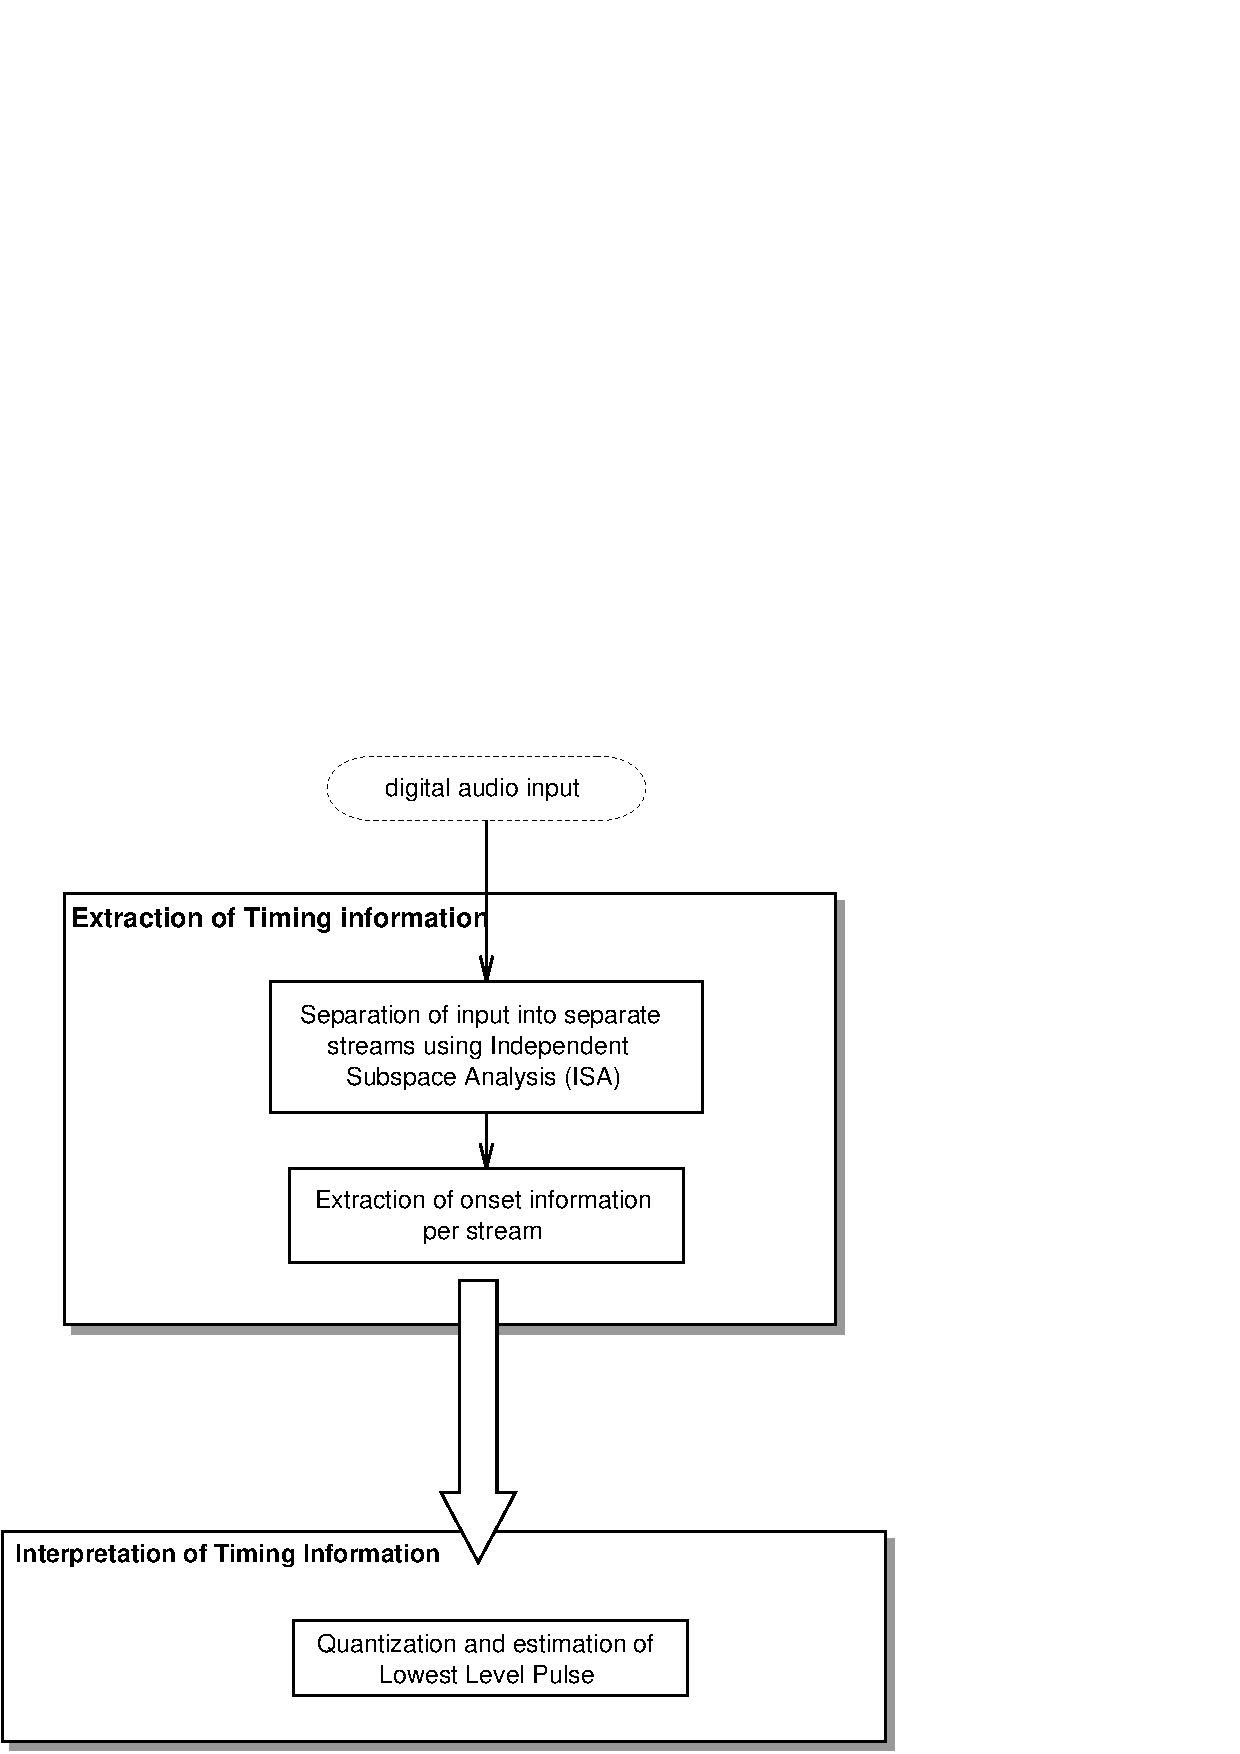
\includegraphics{SystemArchitecture.pdf}}
    \caption{Riddim: The System Architecture }
    \label{system architecture}
  \end{center}
\end{figure}

Each stream is then passed in succession to an onset detection module.
In this module, a rectify and smooth algorithm is implemented to
prepare the signal for subsequent analyses. Next, a peak detection 
routine finds the points in the stream that correspond to an onset
time or an attack point. The onset detection module will 
return a vector of onset times for each stream that it processes. The 
second high-level subsystem takes in each vector of times from the onset
detection component of the first subsystem, quantizes it and returns the 
lowest level grid for each stream. 

\vspace{5mm}
\subsection{The MATLAB{\texttrademark} Platform}

I chose the MATLAB{\texttrademark} programming language and 
environment as a development platform for my work for several reasons.
First of all it is a common platform for prototyping complex systems,
with widespread support among scientists and engineers, in industry
and academia. It has numerous highly specialized toolboxes for 
mathematical analyses and design in a variety of disciplines. 
This makes it an attractive tool for solving problems quickly, 
more so than a tool to build a commercial application.

Another motivation for using MATLAB{\texttrademark} came from the fact
the implementation of Casey's Independent Subspace Analysis
(ISA) was in MATLAB{\texttrademark}.  Since this was work that formed a 
central part of my application and was one that I intended to use ``as is'' 
with very only minor functional modifications, it made sense to build 
the rest of my application on the same platform.

\vspace{5mm}
\subsection{Native C subroutines via the MEX interface}

However, not all modules were written in MATLAB{\texttrademark}. 
MATLAB{\texttrademark} provides an Application Programmer's 
Interface (API) called MEX that permits external subroutines written in 
C or Fortran to be called from MATLAB{\texttrademark} functions, 
script files or the command line. These special C subroutines are
compiled into MEX-files which are dynamically linked subroutines 
that the MATLAB{\texttrademark} interpreter can load and execute.

Several parts of this work were implemented in C and called via
the MEX interface. These include the bulk of the onset detection 
module and sections of the grid quantization modules.
The main advantages of implementing certain functionality in C is 
speed.  Since MATLAB{\texttrademark} is an interpreted language optimized for 
vector operations, certain constructs like \texttt{for} or \texttt{while} 
loops can be very slow for very large arrays. In such cases, to
increase the overall performance, such operations can be implemented
in C. Another motivation came from the fact that several authors 
sent me demos of their algorithms as MATLAB{\texttrademark}
functions. On one hand it would have been easy to simply use their
code in my implementation. However, to really internalize their work,
I felt that it was important to come up with my own implementation in C.


\vspace{7mm}
\section{Independent Subspace Analysis}
\vspace{3mm}

\subsection{Motivation}

If the goal was to implement a tool that can extract rhythmic 
information from digital audio, what would be the best way to decompose 
the data to facilitate an analysis? How does the brain focus its
attention on a singular element in a sound mixture to be able to pick
out its rhythmic qualities? Does a model of attention really help? 
Is any decomposition or data  reduction even necessary? 

According to Leigh Smith ``The perception  of musically typical rhythms is achieved by 
segregation of the received sound complex into separate streams of 
common sources. It is thereby hypothesized that listeners use timbral, spatial 
localisation, pitch, tempo and other objective differences between 
sound sources to distinguish between independent rhythmic patterns'' \cite[p .85]{Smith:99}.
A first step in implementing a robust perceptual rhythm analysis 
tool is to find a scheme that permits monophonic audio sources to be 
segregated or ``un-mixed'' into their source streams.  In the past, this
problem in the past has been notoriously difficult to solve \cite{Bilmes:93}.
This may be due in part to the characteristic representation of the 
audio signal, the fact that perceptually, sound qualities such 
as timbre and pitch are still evasively difficult to quantify 
accurately and the ``heuristic nature of psycho-acoustic 
grouping rules'' \cite{Casey:2000}.  

First of all, we will discuss some important notions necessary 
to a complete understanding of ISA.

\subsection{The Mechanics of Mixing and Unmixing}

Let us assume that we have two different recordings of an event
involving two instruments. We want to recover the two individual 
instruments which are mixed in varying degrees in the recordings. 

In this simple case, we have two {\it observed} or {\it recorded} 
sounds that we call $y_{1}(t)$ and $y_{2}(t)$, each $n$ samples long. 
We write them in row vector form as, 

\begin{figure}[thp]
  \begin{center}
    \resizebox{4in}{!}{\includegraphics{PDFHistoWaveform.pdf}}
    \caption{The waveform (time-series) representation of several
      conga hits 451 samples long.} 
    \label{PDFHistoWaveform}
  \end{center}
\end{figure}

\begin{figure}[thp]
  \begin{center}
    \resizebox{4in}{!}{\includegraphics{PDFHisto.pdf}}
    \caption{A histogram representation of Figure
      \ref{PDFHistoWaveform} that approximates a probability density
      function close to a spiky Gaussian.}
    \label{PDFHisto}
  \end{center}
\end{figure}

\begin{equation}
  \label{twoobservedsounds}
  \matrix{
    y_{1}(t) = [y_{1}(1),...,y_{1}(n)] \cr
    y_{2}(t) = [y_{2}(1),...,y_{2}(n)] \cr
    & }
\end{equation}
These observed sounds contain a mixture of sounds from different
instrument sources that we call $x_{1}(t)$ and $x_{2}(t)$ which are also 
$n$ samples long each and are written as,

\begin{equation}
  \label{twolatentsounds}
  \matrix{
    x_{1}(t) = [x_{1}(1),...,x_{1}(n)] \cr
    x_{2}(t) = [x_{2}(1),...,x_{2}(n)] \cr
    &}
\end{equation}
Because of the relatively high sampling rate of the sounds, we can 
represent $x_{1}(t)$ and $x_{2}(t)$ in a histogram of the signals'
amplitudes. The shape of the histograms are a good approximation of 
the probability density functions (PDF) $P(X_{1})$ and $P(X_{2})$ of 
a pair of random variables $X_{1}$ and $X_{2}$. Later we will be
making assumptions about the characteristics of these PDFs.

For notational purposes, we put each pair of vectors into $2
\times n$ matrix so $$ X = \left [
  \matrix{
    x_{1}(t)  \cr
    x_{2}(t)  \cr
    }
\right ] \hbox{ and } Y = 
\left [
  \matrix{
    y_{1}(t)  \cr
    y_{2}(t)  \cr
    }
\right ] $$
[Note that $X$ is not directly related to $X_{1},X_{2}$ defined above.]
There are two assumptions that we take the liberty of making in
discussing how $x_{1}(t)$ and $x_{2}(t)$ are combined to yield $y_{1}(t)$ 
and $y_{2}(t)$. The first assumption is that $x_{1}(t)$ and $x_{2}(t)$
in $X$ are linearly mixed. This means that $Y$ is the product of $X$
and some full rank mixing matrix $M$, 
\begin{equation}
  \label{mixing}
  Y = MX
\end{equation}
where the $M$ realizes the linear mixing.  Thus to recover $X$ given
$Y$ reduces to left multiplying $Y$ by the $M^{-1}$,
\begin{equation}
  \label{unmixing}
  X = M^{-1}Y
\end{equation}
In our situation, pulling recordings from CDs or vinyl, we have 
the mixture $Y$ and we don't know $M$. Thus to recover the sources $X$
we must try to estimate $M^{-1}$ from the mixture $Y$. 
To help this estimation, a second assumption is made. This is that 
random variables $X_{1}$ and $X_{2}$ (introduced above), whose PDFs are
modeled by the histograms of $x_{1}(t)$ and $x_{2}(t)$ respectively, are 
{\it independent}.  This means that their joint probability
distribution given by,
\begin{equation}
  \label{independence}
  P(X_{1},X_{2}) = P(X_{1}) \cdot P(X_{2})
\end{equation}
is separable. Plotting the histogram for two sound sources that are
independent with uniform distributions we see that ideally their 
joint distribution is square-like. On the other hand,
plotting the histograms for two highly correlated sounds, we see that
their joint distribution tends to run along an axis. 

\begin{figure}[thp]
  \begin{center}
    \resizebox{5in}{!}{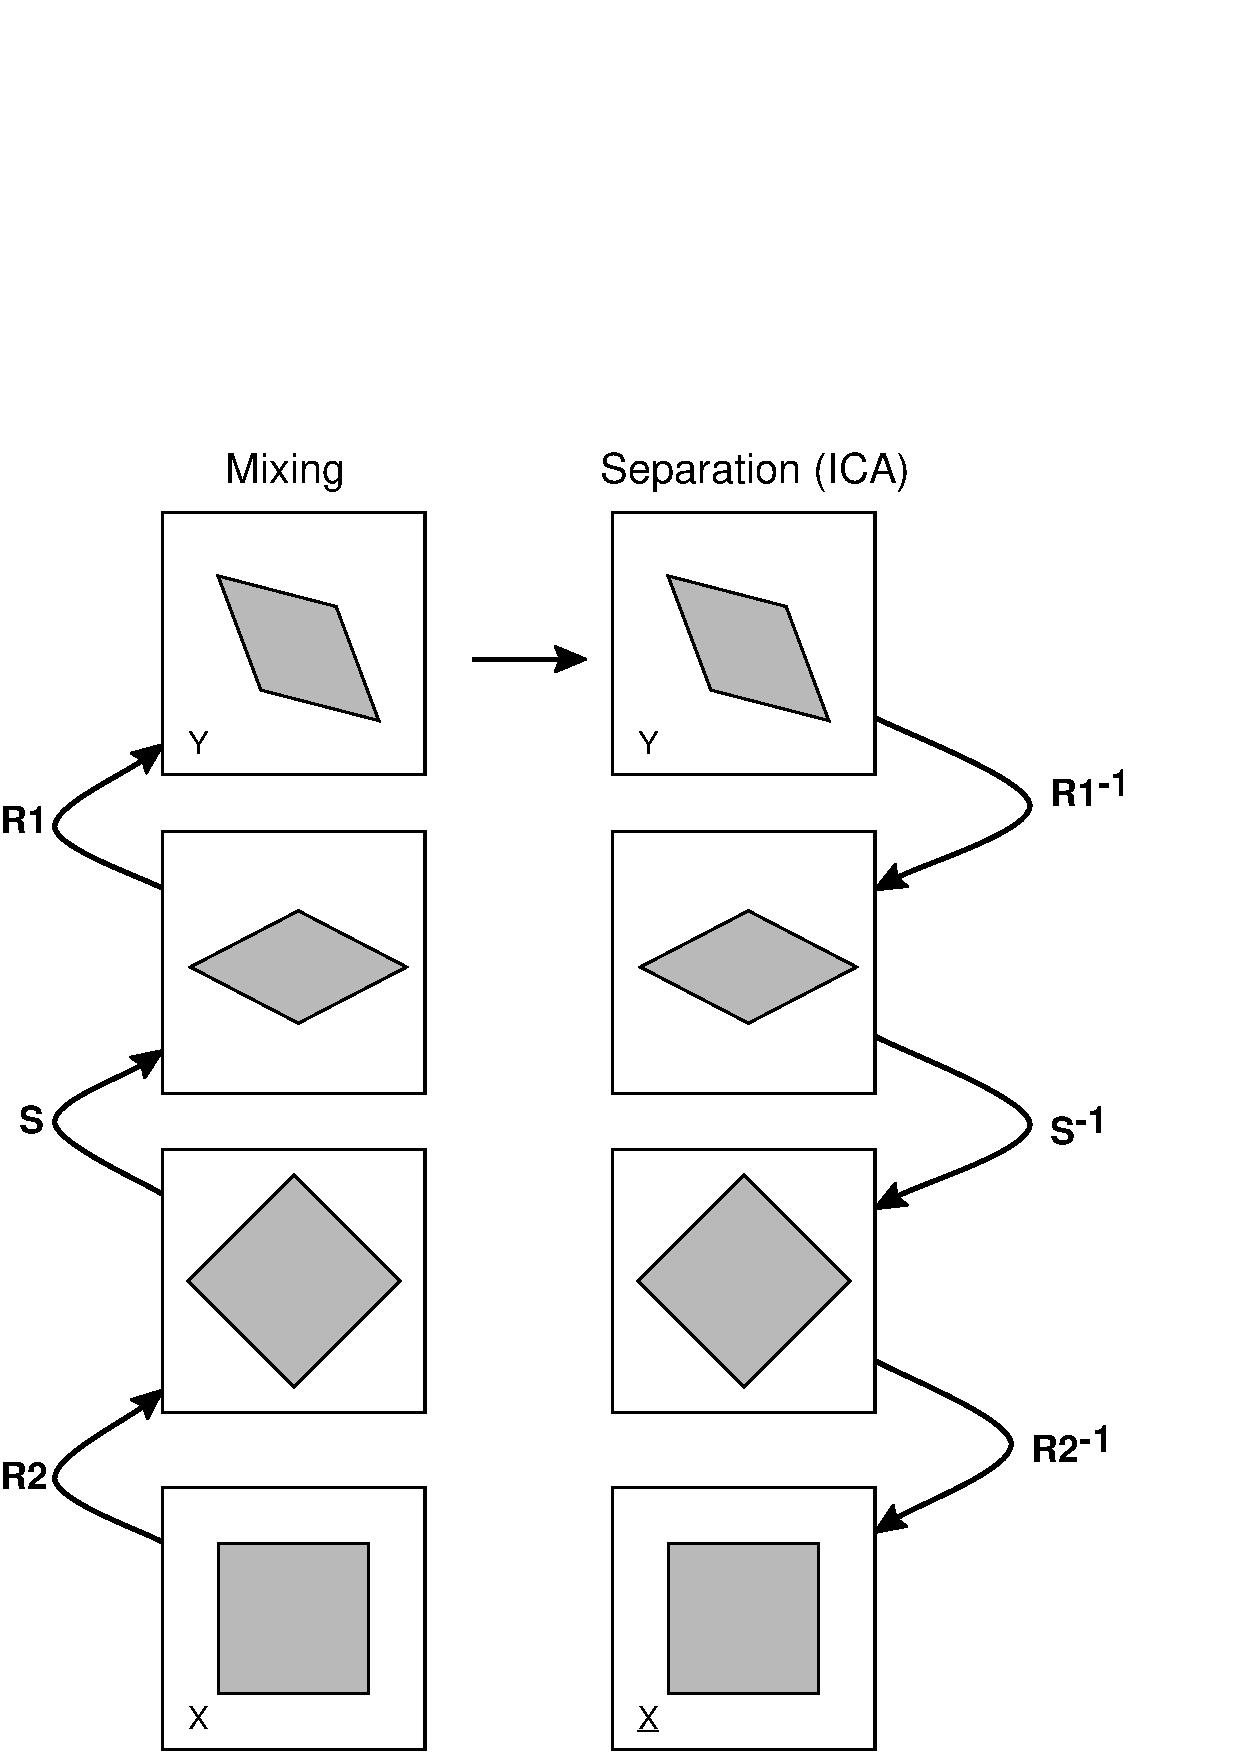
\includegraphics{MixingUnMixing.pdf}}
    \caption{From \cite{Farid:99}, the bottom left shows an
      ideal joint probability density function of two independent
      signals in $X$. The linear mixing of the signals in equation
      \ref{mixing} transforms the distribution by rotating 
      it with $R_{2}$, scaling it with $S$ and rotating it with
      $R_{1}$. ICA tries to estimate $M^{-1}$ by finding rotation
      matrices $R_{1}^{-1}$ and $R_{2}^{-1}$, and scaling matrix
      $S^{-1}$ that transforms the joint PDF of the mixed signals back to a
      square.}
    \label{MixingUnmixing}
  \end{center}
\end{figure}

\vspace{5mm}
\subsubsection{Decomposing the Mixing Matrix}

From equation \ref{mixing}, one can gain some intuition into the
mechanics of the mixing procedure by diagonalizing the matrix $M$.
Using the Singular Value Decomposition (SVD), $M$ can be expressed as 
\begin{equation}
  \label{SVD}
  M = R_{1}SR_{2}
\end{equation} where $R_{1}$ and $R_{2}$ are orthonormal matrices and
$S$ a diagonal matrix \cite{Farid:99}. Figure \ref{MixingUnmixing}
shows that $M$ applied to the idealized joint distribution of a pair of independent
signals can be seen as matrix $R_{2}$ performing a rotation, diagonal
matrix $S$, a scaling, and $R_{2}$ a final rotation to yield the 
joint PDF of the mixed signals.

Thus estimating $M^{-1}$ from equation \ref{unmixing} reduces to
finding rotation and scaling matrices that undo the mixing operations.

\vspace{5mm}
\subsection{Principle Component Analysis}

The matrices, $R_{1}^{-1}$ and $S^{-1}$, that perform the
first two inverse operations respectively from Figure
\ref{MixingUnmixing} are obtained via a technique called Principal 
Components Analysis (PCA). PCA inspects the variance structure of 
the data looking for components that account for most of the variation
in the data. It is about the axis of greatest variance that the joint
PDF of the mixed signals (in the upper right corner of Figure \ref{MixingUnmixing}) is
first rotated. This matrix $R_{1}^{-1}$ is obtained first by
calculating the covariance matrix of $X$, written as,
\begin{equation}
  \label{covariance}
  {\bf C}  = XX^{T}
\end{equation}
Next, ${\bf C}$ is diagonalized using SVD to yield three new matrices \cite{Strang:93},
\begin{equation}
{\bf C} = UDV^{T}
\label{SVDCovariance}
\end{equation}
In a zero mean data set, the axis of maximum variance is given by the 
eigenvector corresponding to the first eigenvalue of the covariance matrix ${\bf
C}$. Refer to Figure \ref{PCA}. Thus from equation \ref{SVDCovariance}, $R_{1}^{-1} = V^{T}$. 

The next transformation matrix we must estimate as part of the
separation process from Figure \ref{MixingUnmixing} is the diagonal
scaling matrix $S^{-1}$. In practice it is given by the diagonal
matrix $D$ in equation \ref{SVDCovariance}, so $S^{-1} = D$. 

\begin{figure}[thp]
  \begin{center}
    \resizebox{3.5in}{!}{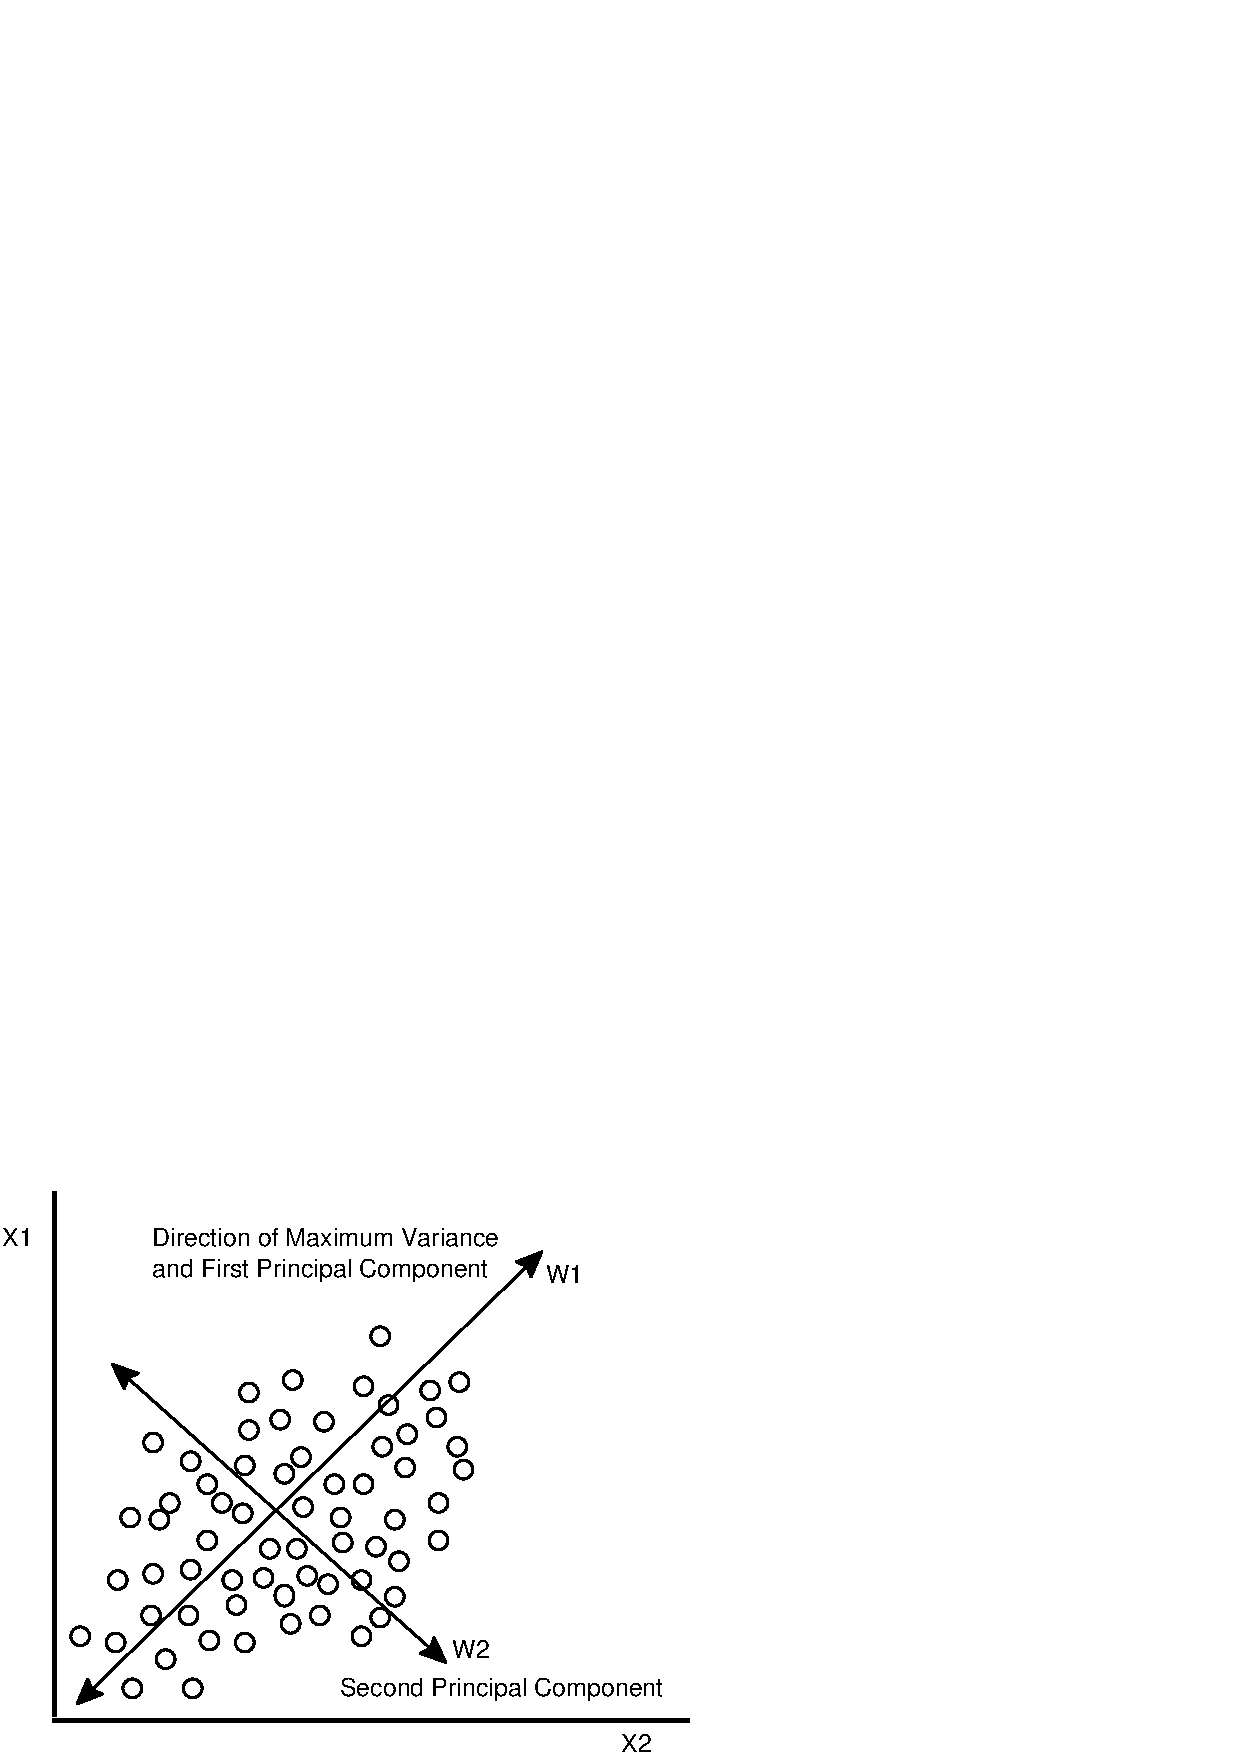
\includegraphics{PCA.pdf}}
    \caption{Principal Component Analysis: $Y1$ and $Y2$ show
      directions of the first two principle components \cite{Cook:97}.}
    \label{PCA}
  \end{center}
\end{figure}

The final rotation matrix $R_{2}^{-1}$ from Figure
\ref{MixingUnmixing} is a bit more difficult to obtain. 
Typically, the angle that transforms the diamond joint PDF into a
square occurs where the kurtosis or fourth-order cumulant of the joint
PDF is minimized. So an error function of the orientation angle of the
joint PDF is defined and local minima of this function across all
orientations angles give a number of possible candidates for
the final rotation matrix $R_{2}^{-1}$ \cite{Farid:99}. 

\vspace{3mm}
\subsubsection{Statistical Independence and Mutual Information}

To narrow down the candidates matrices to one, we
must go back to an initial assumption from equation
\ref{independence}. Here we claimed that the joint PDF of two 
random variables is the same as the product of their PDFs
when the variables are independent. Generalizing equation
\ref{independence} for $N$ variables instead of two, statistical independence
is given by,
\begin{equation}
\label{statisticalIndependence}
P(X_{1},\cdots,X_{N}) = \prod_{i = 1}^N P(X_{i})
\end{equation}
Statistical independence is achieved when the distance between the
joint PDF and the product of the marginal PDFs is minimized.
To calculate distances between PDFs, a measure like the
Kullback-Leibler divergence is used, given for two PDF $P(X), Q(X)$
by, 
\begin{equation}
\label{generalKL}
K(P||Q) = \int P(X)log \Biggl( { P(X)\over Q(X)} \Biggr) dX
\end{equation}
Furthermore, if the probability density function of a mixture factors
into the product of the marginal densities (statistical independence)
the mutual information between the output joint density and the
component densities is said to be zero. 

Thus, by applying each of the candidate rotation matrices obtained
from the local minima of the error function minimizing the kurtosis 
of the joint distribution, the mutual information is calculated. 
The matrix that has the lowest measure of mutual information between 
the joint PDF and the product of the marginal PDFs obtained from its
application to the joint PDF becomes final rotation matrix
$R_{2}^{-1}$ in Figure \ref{MixingUnmixing}.

In practice, though as was mentioned above, the PDFs are approximated 
by the histogram representation of the mixed and individual signals. 

\vspace{5mm}
\subsubsection{Summary}

\begin{figure}[thp]
  \begin{center}
    \resizebox{3.75in}{!}{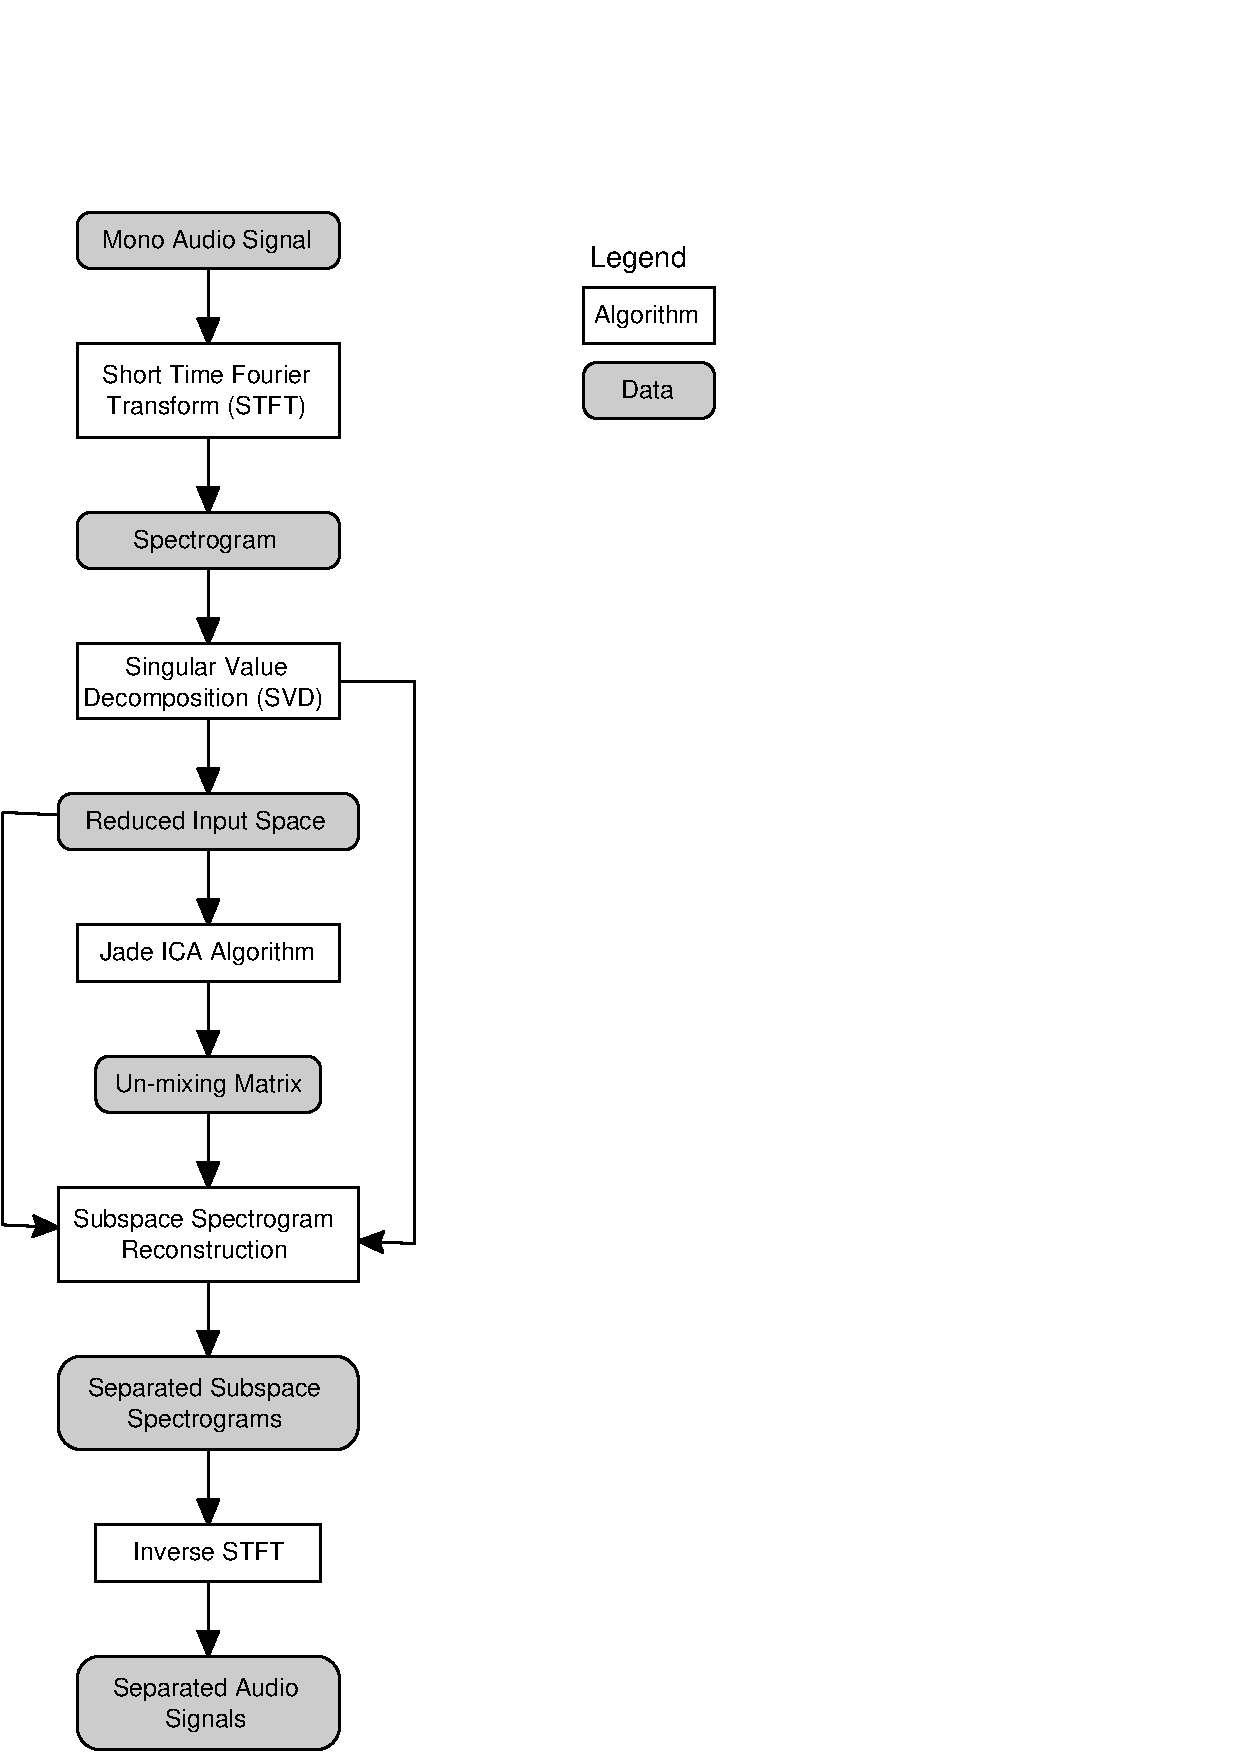
\includegraphics{ISAGeneral.pdf}}
    \caption{High Level Functional Blocks of the ISA Algorithm}
    \label{ISAGeneral}
  \end{center}
\end{figure}

The notion of independence is of central importance to this separation
scheme. Ideas on independence are heavily influenced by Gestalt 
grouping rules and Bregman's views on stream segregation in auditory scene
analysis \cite{Bregman:90}\cite{Casey:2000}. Described above are the
mechanics of one approach to solving the canonical separation problem
using ICA. There are a variety of algorithms in the literature that
use ``higher-order statistics, minimum mutual information or maximum
entropy in their solutions'' \cite{Knuth:98}.

For a more in-depth discussion on independence, mutual information,
ICA algorithms and their derivations, please refer to \cite{Knuth:98}\cite{hyvarinen:99survey}\cite{smaragdis:97}\cite{Farid:99}\cite{Casey:2000}.

\vspace{5mm}
\subsection{Independent Subspace Analysis}

Casey's innovation in ISA was the idea to take a mono signal (that
ordinarily cannot be un-mixed directly using ICA) and perform
a change of basis operation before employing canonical ICA techniques.
A mono signal of size $1 \times N$ is first projected onto a new bases of sines and
cosines using a windowed Short Time Fourier Transform (STFT) to yield
a spectrogram of size $n \times m$. This new multidimensional manifold
is composed of $m$ time slices each containing $n$ frequency bins.
\begin{figure}[thp]
  \begin{center}
    \resizebox{5in}{!}{\includegraphics{ISAflow.pdf}}
    \caption{Details of the ISA algorithm}
    \label{isaflow}
  \end{center}
\end{figure}
The general approach is to do a dimension reduction on this
high dimension space to obtain a reduced set of vectors spanning the
input space. This is accomplished by performing SVD on the covariance
matrix of the input spectrogram. The input spectrogram is then
projected onto this new basis to yield a dimension-reduced input space.
The input basis vectors are then fed to the Jade\footnote{Jade is an
ICA algorithm by Jean-Fran{\c c}ois Cardoso} algorithm which returns
the mixing matrix $A \approx M^{-1}$.  The un-mixing matrix is then 
multiplied against the dimension-reduced basis vectors from the 
spectrogram projection to yield the independent components oriented in time.  

\begin{landscape}
  \begin{figure}
    \centering
    \includegraphics[width=7in]{ZingZongOriginal.pdf}
    \caption{A waveform of an eight second excerpt of a recording of
      Soukous music from the Congo}
    \label{zingzongoriginal}
  \end{figure}
\end{landscape}

\begin{landscape}
  \begin{figure}
    \centering
    \includegraphics[width=7in]{ZingZongExtractedKick.pdf}
    \caption{The extracted kick drum from the Soukous music}
    \label{zingzongkick}
  \end{figure}
\end{landscape}

\begin{landscape}
  \begin{figure}
    \centering
    \includegraphics[width=7in]{ZingZongExtractedSnare.pdf}
    \caption{The extracted snare drum from the Soukous music}
    \label{zingzongsnare}
  \end{figure}
\end{landscape}

\begin{landscape}
  \begin{figure}
    \centering
    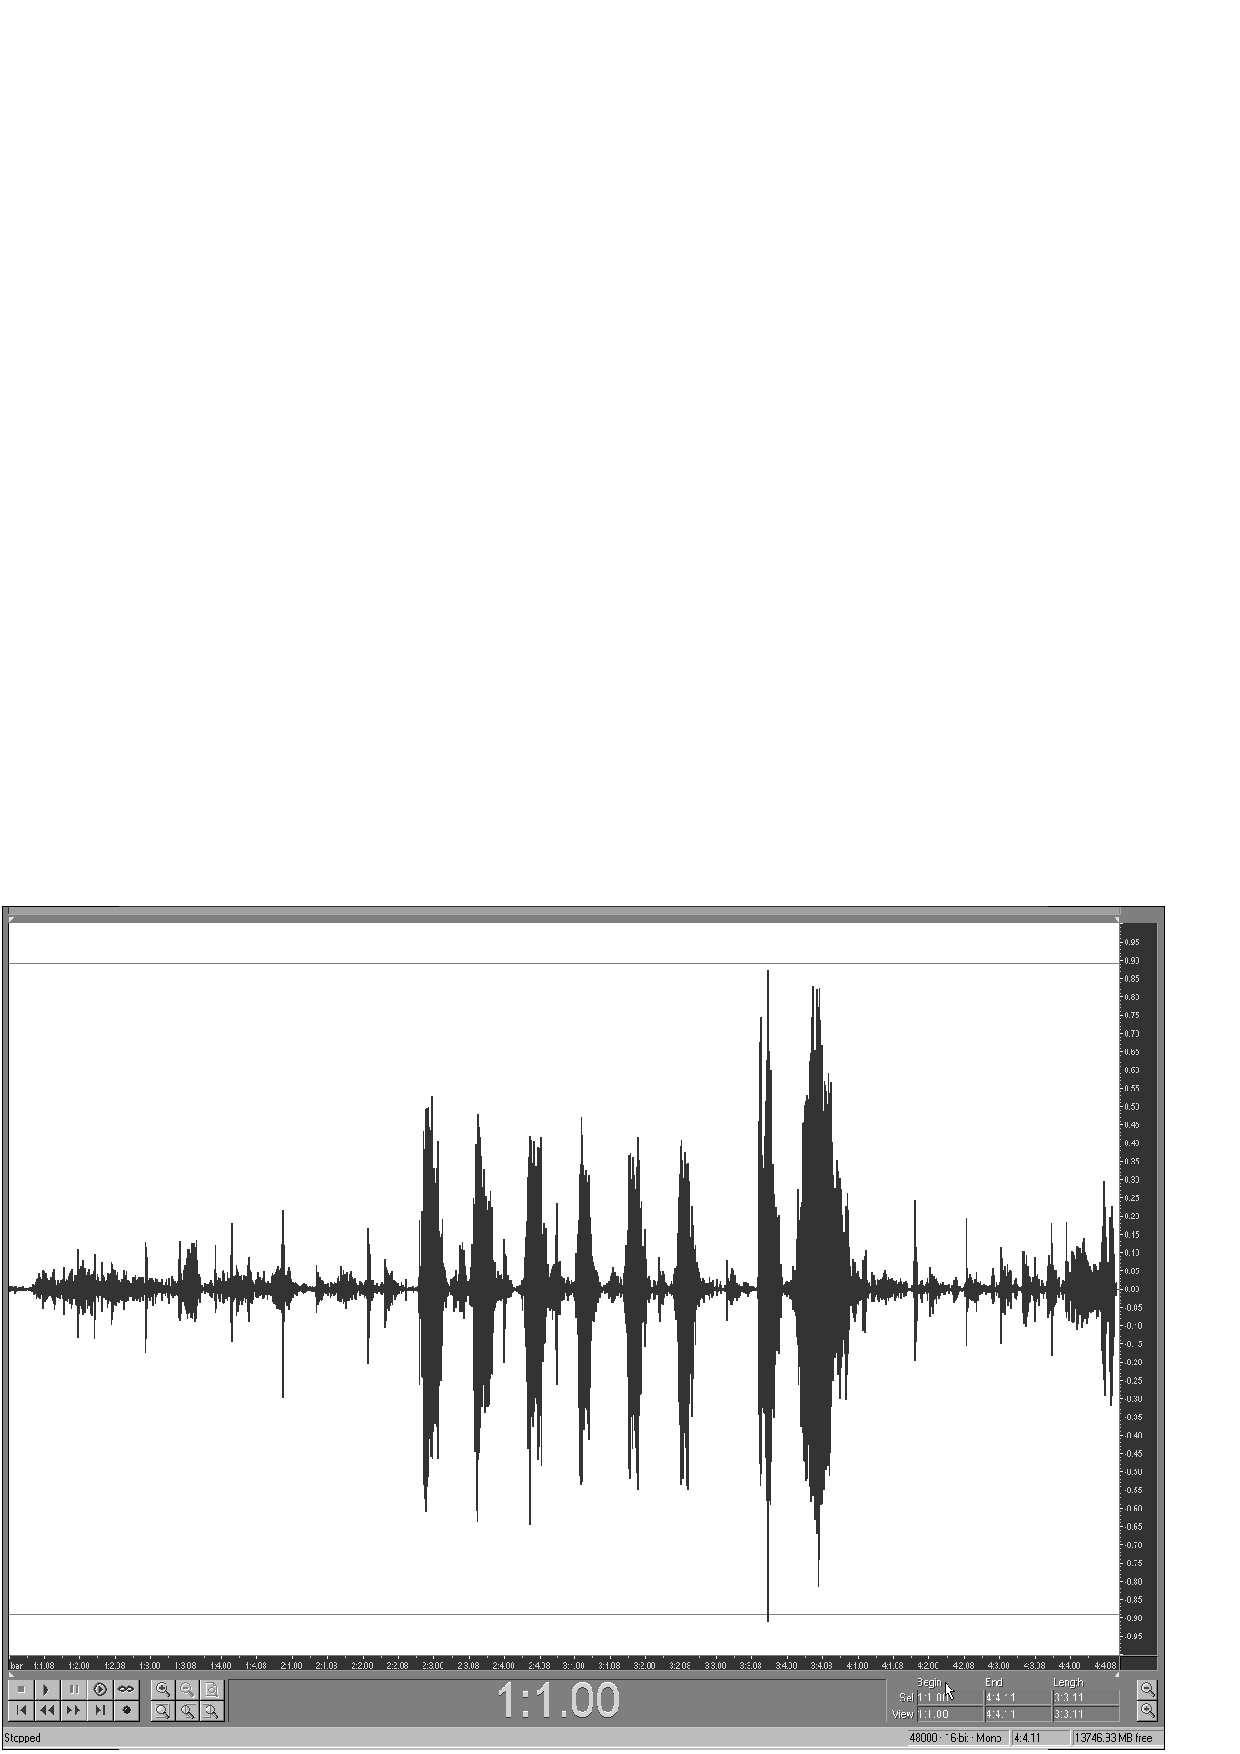
\includegraphics[width=7in]{ZingZongExtractedVox.pdf}
    \caption{The extracted human vocal chants from the Soukous music}
    \label{zingzongvox}
  \end{figure}
\end{landscape}

\begin{landscape}
  \begin{figure}
    \centering
    \includegraphics[width=7in]{ZingZongExtractedWhistle.pdf}
    \caption{The extracted whistle blow from the Soukous music}
    \label{zingzongwhistle}
  \end{figure}
\end{landscape}

Next, frequency varying weights for each independent component are 
calculated by multiplying the un-mixing matrix against the SVD reduced
vectors. Together, the basis vectors and the frequency varying weights
are combined to yield individual subspace spectrograms corresponding
to independent marginal distributions within the original
time-frequency space. These spectrograms are then passed through a 
windowed inverse STFT (ISTFT) to yield the time domain audio signals 
corresponding to the extracted streams. 

\vspace{7mm}
\section{Detecting Onset Points}
\vspace{3mm}

The next subsystem in the processing chain extracts onset timing
information from each of the audio streams passed to it. The onset detection
algorithm used was taken from a paper on sound segmentation by 
Anssi Klapuri \cite{Klapuri:99} at Tampere University of Technology 
(TUT) in Finland.

Onset detection is based on the fact that humans are built to detect real-world
structure by detecting changes along physical dimensions, representing
the changes as relations \cite{Jones:76}.

Researchers in sound segmentation and onset detection agree that
a robust system should imitate the human auditory system by treating
frequency bands separately and combining onset information from each
band at the end of the analysis. 
\begin{figure}[thp]
  \begin{center}
    \resizebox{3in}{!}{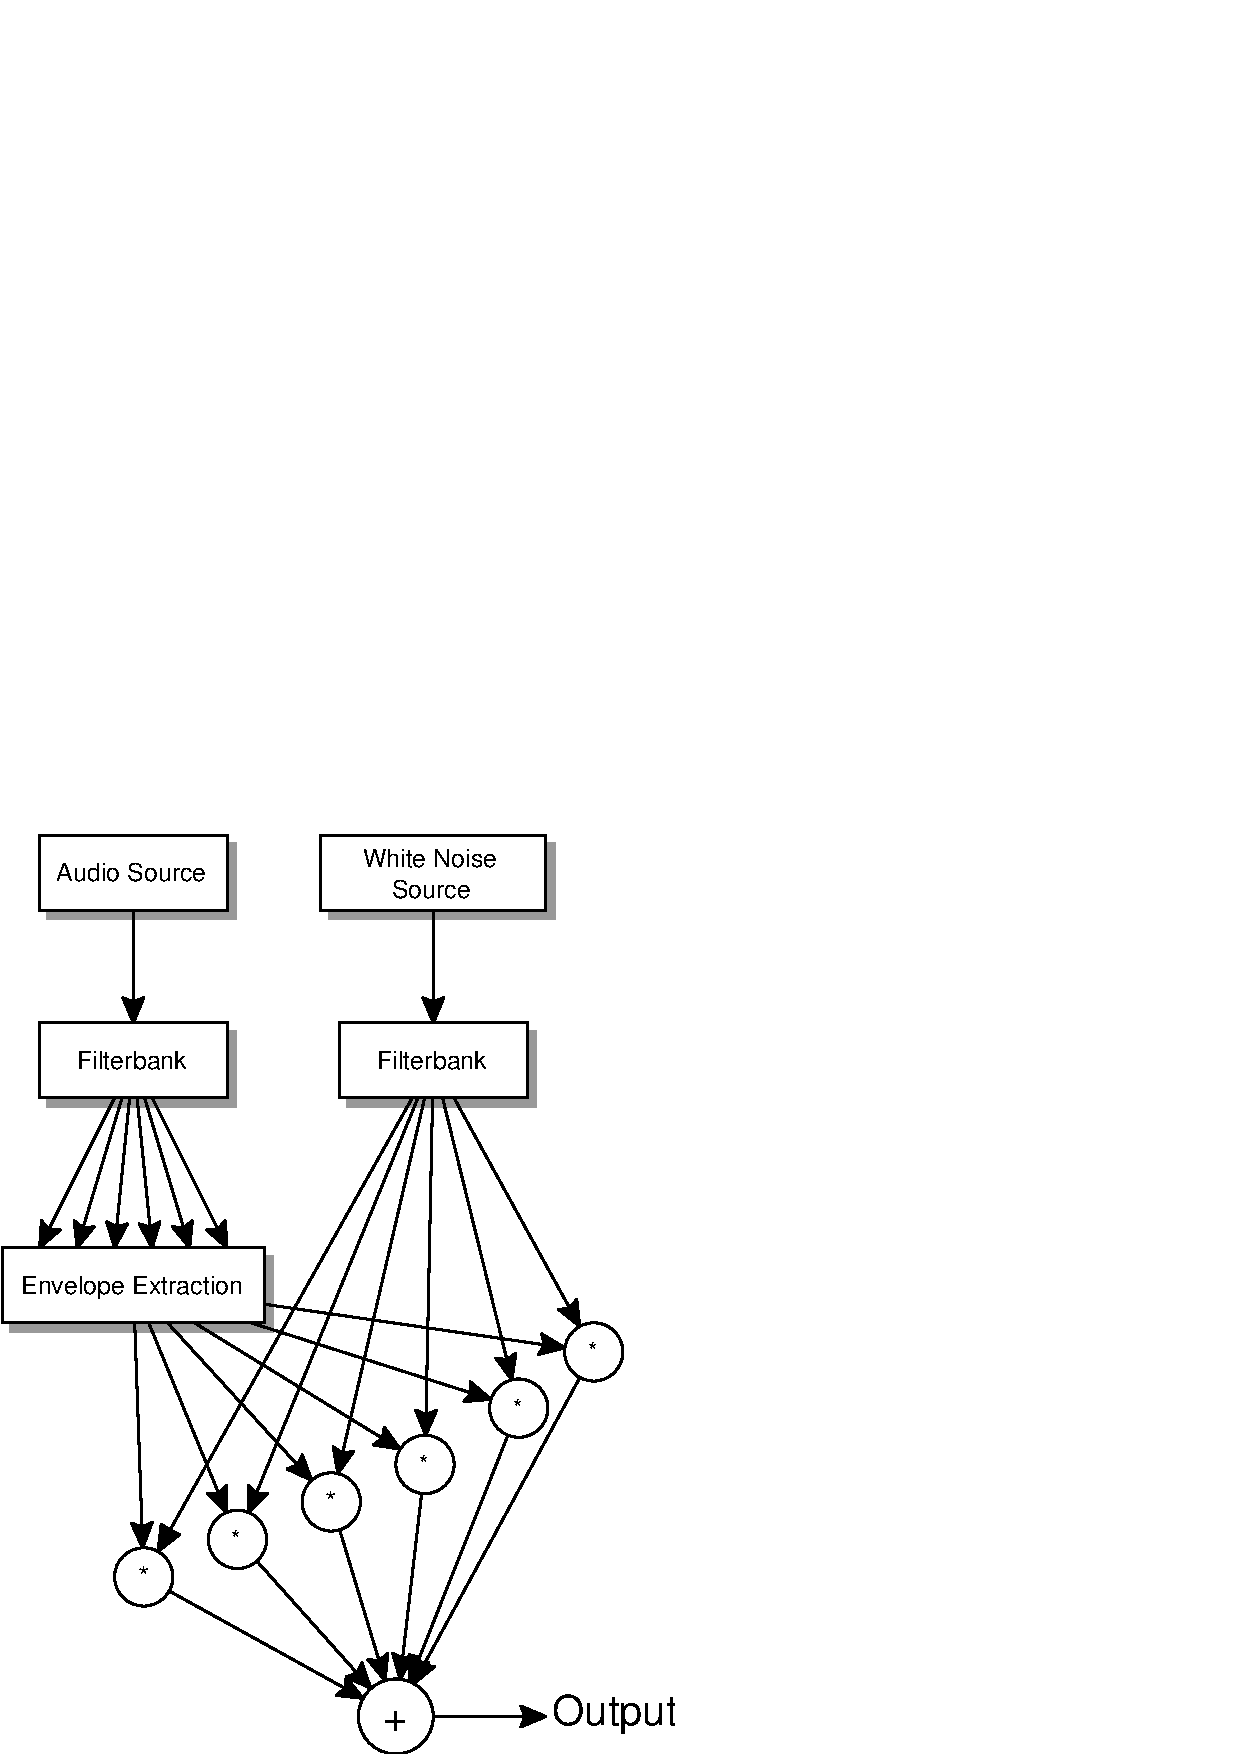
\includegraphics{AmpNoiseEnvelope.pdf}}
    \caption{``Amplitude Modulated'' white noise from a musical signal
      has the same rhythmic percept as the signal}
    \label{AMod}
  \end{center}
\end{figure}
The first detection systems tried to analyse the amplitude envelope of
the audio signal as a whole without any band filtering.  Since the
results were not very accurate, researchers moved to concurrent
analyses in different frequency bands combining the various
band results at the end \cite{Klapuri:99}\cite{Scheirer:98tempo}.
In a sense, separately processing frequency bands crudely imitates the human
auditory system's tuning curves. This approximation becomes
unnecessary when individual streams are separated. Thus, in my
implementation of Klapuri's onset tracking algorithm, I do not preprocess
the extracted streams through any filterbanks, but analyse each stream as is.  

Another psychoacoustic principle that is employed to simplify 
the onset detection algorithm deals with the perceptual rhythmic 
proximity of an amplitude modulated noise signal to the original signal. 
One can construct an amplitude-modulated noise signal by passing 
a white noise signal and a musical signal through the same set of 
filter banks. The amplitude envelope of the output of each of the 
music signal filter banks is used to control the corresponding noise 
band amplitude. The resulting noise signals are then summed together
to form an output signal. Refer to Figure \ref{AMod}.

Scheirer reports that ``when an audio signal is divided into  
at least four frequency bands and the corresponding bands of a 
noise signal are controlled by the amplitude envelopes of the 
musical signal, the noise signal will have a rhythmic percept 
which is significantly the same as that of the original signal'' \cite{Scheirer:98tempo}. 
The importance of this is that since ``the only thing preserved in this
transformation is the amplitude envelopes of the filter bank outputs,
it stands to reason that only this much information is necessary to
extract pulse and meter from a musical signal; that is, algorithms for
pulse extraction can be created which operate only on this much input
data and ``notes'' are not a necessary component for hearing rhythm'' \cite{Scheirer:98tempo}. 

The importance of this psychoacoustic simplification is that the
task of finding rhythmically significant time points in a section of
audio reduces to finding the same points on a drastically smaller data
set, i.e. the smoothed amplitude envelope of that same section of
audio. This smoothed version of the original is attained via a
rectification and smoothing algorithm.

\begin{landscape}
  \begin{figure}
    \centering
    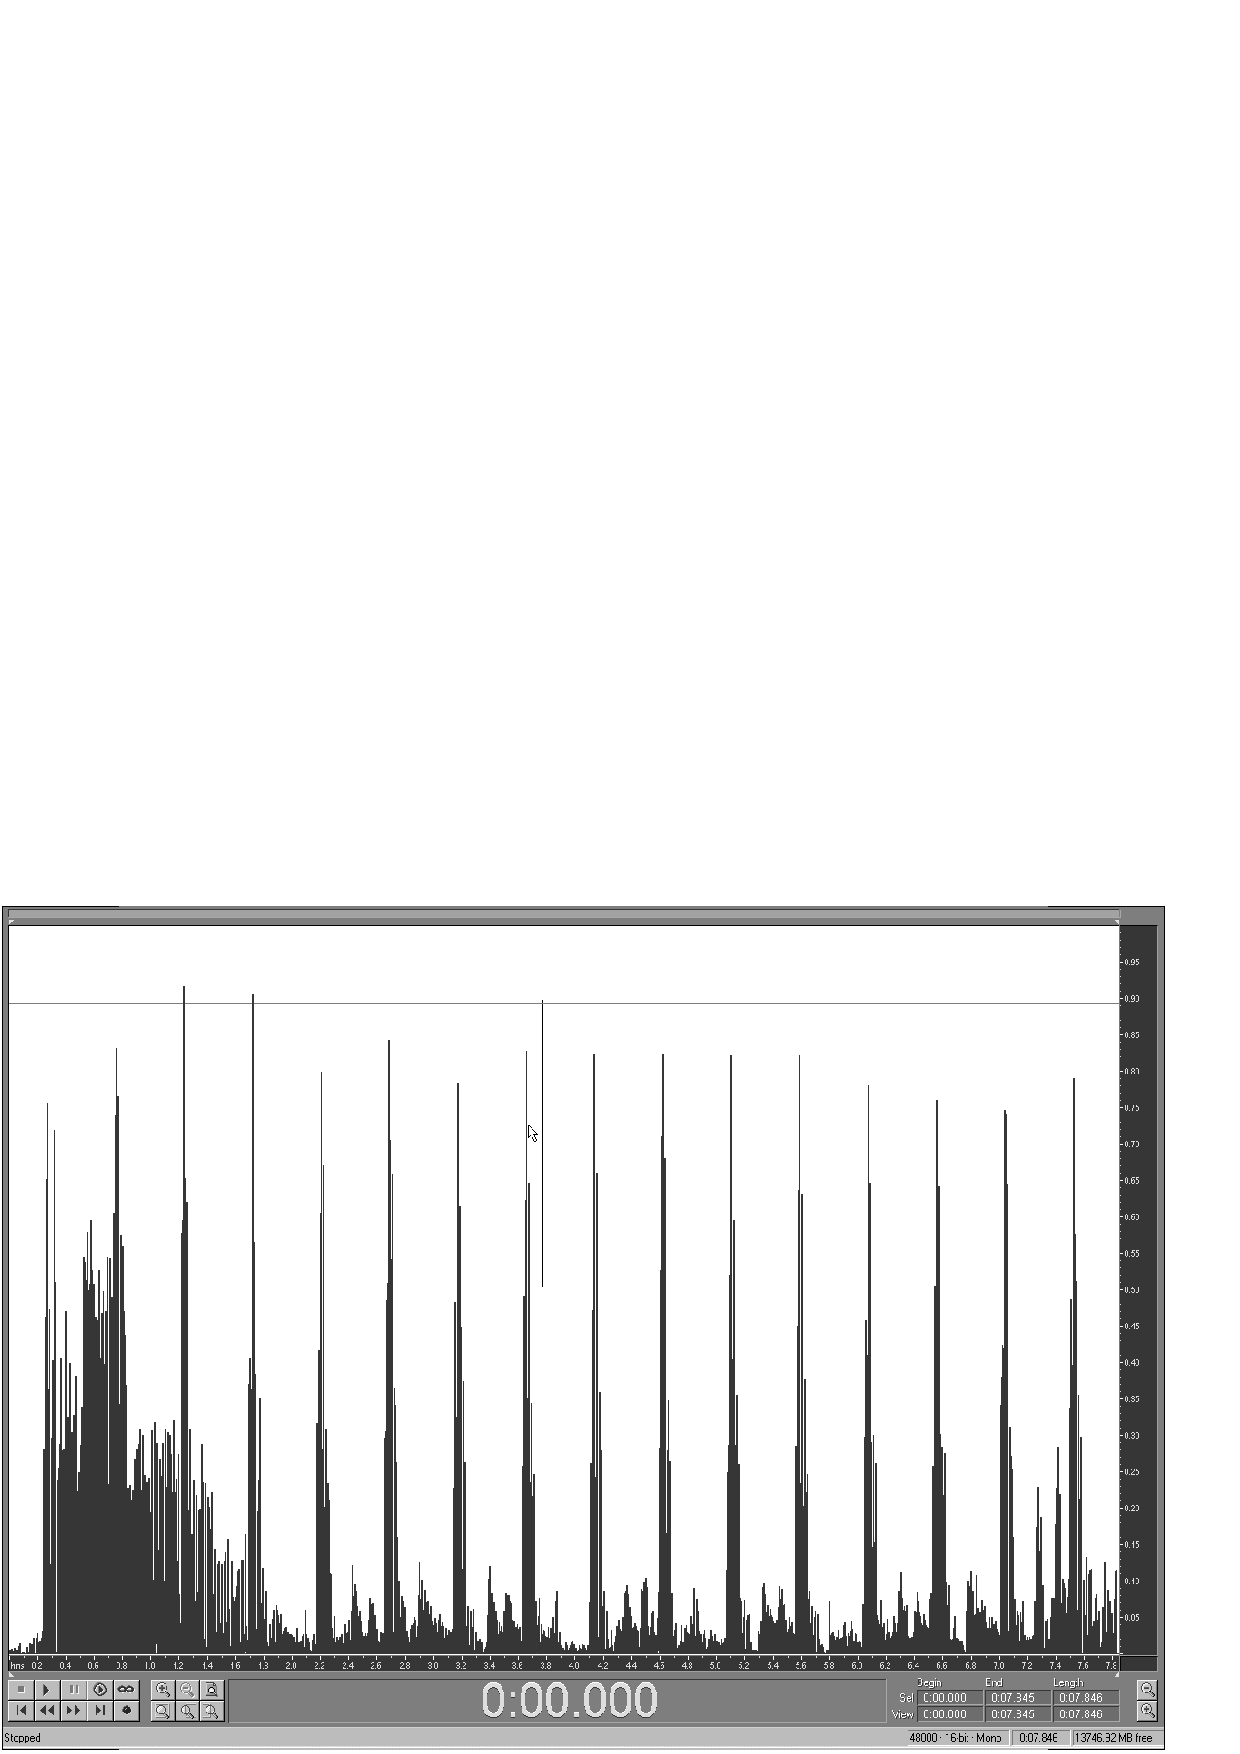
\includegraphics[width=7in]{ZingZongKickRectified.pdf}
    \caption{The soukous kick drum after its been half-wave rectified}
    \label{kickrect}
  \end{figure}
\end{landscape}

\vspace{5mm}
\subsection{Rectification and Smoothing}

From an audio signal with potentially cumbersome imperfections our task is to prepare 
the signal for a robust peak searching algorithm by first applying a
rectify-and-smooth algorithm proposed by Scheirer \cite{Scheirer:98tempo}.
First, the input audio stream is half-wave rectified. This means that all the
negative bits of the signal cycle are converted to zero. Refer to
Figure \ref{zingzongkick} and \ref{kickrect} for a graphical representation of
what occurs before and after rectification.

At this stage, the rectified signal is decimated. This involves a two
step process in which the signal is low pass filtered with a sixth
order Chebyshev Type I lowpass filter with a cutoff frequency,
$$w = {.8(\hbox{ samplerate}) \over 2R}$$ where $R$ is the decimation factor. The
second part of the decimation process is the actual resampling of the
signal at $1/R$ its original rate.  Decimation is implemented to allow
all further operations on the data to be more computationally
efficient, since there is minimal data loss for signals with sample
rates as high as $44100 \ samples/second$.

The decimated signal is then convolved with a 200 msec raised cosine 
window.  The window's discontinuity in time (i.e. the start and end 
points are not at the same level) means that its Fourier transform 
has a non-linear phase response. This means that lower frequencies are 
passed through with a larger delay than higher ones.  The window
has low pass filter qualities with a -10dB response at 10Hz and $6
dB/octave$ rolloff afterwards. It performs a kind of energy integration
similar to what occurs in the ear by weighting the most recent inputs
and masking rapid amplitude modulations in the signal.  The net effect
of convolving the input data with this window is that all the rough 
edges, discontinuities, rapid modulations and other ``imperfections'' 
in the signal are smoothed and we are left with just the amplitude 
envelope of the original signal \cite{Scheirer:98tempo}. 


\vspace{5mm}
\subsection{Amplitude Envelope Peak Detection}

Once the signal has been suitably smoothed, it is now time to search
for peaks or sudden changes in signal intensity or representative
sound pressure level that would suggest the presence of an attack
point or onset.  Most algorithms from the literature accomplish this 
task in one way or another by examining peaks in the first order 
difference (FOD) function of the original signal, which correspond 
to the points on the signal with the steepest positive slope. For a 
time domain signal S(t) the first order difference function FOD can 
be defined as: 
\begin{equation}
FOD(t) = {1 \over \Delta t} (S(t) - S(t-1))
\label{FOD}
\end{equation}

\begin{figure}[thp]
  \begin{center}
    \resizebox{4in}{!}{\includegraphics{SlowlyOnsettingSound.pdf}}
    \label{A Slowly Onsetting Sound}
    \caption{When using peaks in the {\sl first order difference
        function} to determine onset times, the estimation is
      sometimes late with slowly onsetting sounds and local maxima may
      be picked as separate onsets.}
  \end{center}
\end{figure}

Klapuri's algorithm is different in several ways that directly address
two problems when using the peaks of the FOD function. First of all,
researchers at TUT noticed that the first derivative measures the
signal loudness well, but the maximum value of the signal's slope does not
correspond directly to the start time of the onset. This is due to the
fact that if the sound takes some time to rise to its maximum value, 
the point at which there is a maximum slope might be late in relation 
to the physical onset of the sound. Note, I refer here to the {\sl
physical onset} not the perceptual onset. The distinction is important
since the physical onset is the one that would be used in a tool like
Recycle{\texttrademark} for splicing and rearranging loops. The
perceptual onset, which is where the human would subjectively mark as the
beginning of the event, may not necessarily coincide with the physical
onset. If the sound rises slowly, its perceptual onset may be
significantly later than the physical onset. Additionally, many sounds
as they rise from do not monotonically increase. There are usually
many local maxima and minima throughout the attack point that may 
be confused as separate attacks \cite{Klapuri:99}.

To handle these problems, Klapuri suggests using the {\sl relative
difference function} (RDF). The RDF in layman's terms is the ratio of the FOD 
to the original signal. It measures the amount of change in
a signal relative to its level and is equivalent to the FOD of the 
logarithm of the signal \cite{Klapuri:99}. 

\begin{equation}
RDF(t) = {1 \over \Delta t}(log(S(t)) - log(S(t-1)))
\label{RDF}
\end{equation}

\begin{figure}[thp]
  \begin{center}
    \resizebox{5in}{!}{\includegraphics{FODvsRDF.pdf}}
    \label{Comparison of First Order Difference and Relative
      Difference Functions}
    \caption{Comparison of the First Order Difference and Relative
      Difference function of a signal, the grid lines correspond to
      peaks in the RDF above a particular threshold}
  \end{center}
\end{figure}

The RDF solves the above mentioned problems since its peaks 
correspond to the beginning of the physical onset, thereby
resolving the problem of late onset estimation with gradually
increasing sounds. Moreover, once a signal starts to rise, local
minima and maxima along the attack slope are not significant relative
to the signal's level.

\begin{figure}[thp]
  \begin{center}
    \resizebox{5in}{!}{\includegraphics{ZingZongOnsetsVoice.pdf}}
    \caption{A separated Soukous vocal chant, gridlines indicate time
      points where onsets are detected. The threshold value is set to .3}
    \label{vocalsampleonsets}
  \end{center}
\end{figure}

So the output of this module returns for each stream it processes, 
a sequence of time values in the stream when the onsets occur. If for
example, an extracted snare drum pattern was passed, 
it will return the start times of each snare hit. This information 
is significant for rhythmic analyses since the difference in start
times or inter-onset intervals (IOIs) are important in the
composition of rhythmic patterns. The snare hit ``off-times'' are less
important from a rhythmic point of view since once the onset occurs
and that attack has happened what follows is less important for the
determination of a rhythmic percept.

During the determination of the peaks in the RDF, the loudness of each
peak is also calculated. The inner or dot product of the FOD
of the signal is taken with a Gaussian window equivalent in length to 
200 msec. The peak of the FOD coincides with the middle point 
of the normal Gaussian window. Refer to Figure \ref{Loudness}.

\begin{figure}[thp]
  \begin{center}
    \resizebox{4in}{!}{\includegraphics{loudness.pdf}}
    \caption{The FOD represents well the loudness of an onsetting
      sound, the loudness is thus calculated by taking the inner
      product of a Gaussian window centered about the FOD peak in question}
    \label{Loudness}
  \end{center}
\end{figure}

After the onsets are obtained as well as their respective sound pressure
levels, the timing data is run through a {\it pruning} routine. Pruning
helps eliminate spurious onsets due to imperfections present in the
ISA separation.  This routine takes the minimum spacing between onsets as
an argument set by the user. While the perceptual limit for
discriminable sounds tends to be around one sixteenth of a second,
percussive flams and grace note flourishes can be much more
rapid. Along with the spacing parameter for pruning, users can also set a
threshold value.  This is useful in dealing with anomalies
in the extracted signal that are usually at a much lower level than the salient
rhythmic features that characterize a stream.  Thus by setting an appropriately high
threshold and a minimum onset interval, clean timing and loudness data
can be gleaned from each stream.

\begin{figure}[thp]
  \begin{center}
    \resizebox{4in}{!}{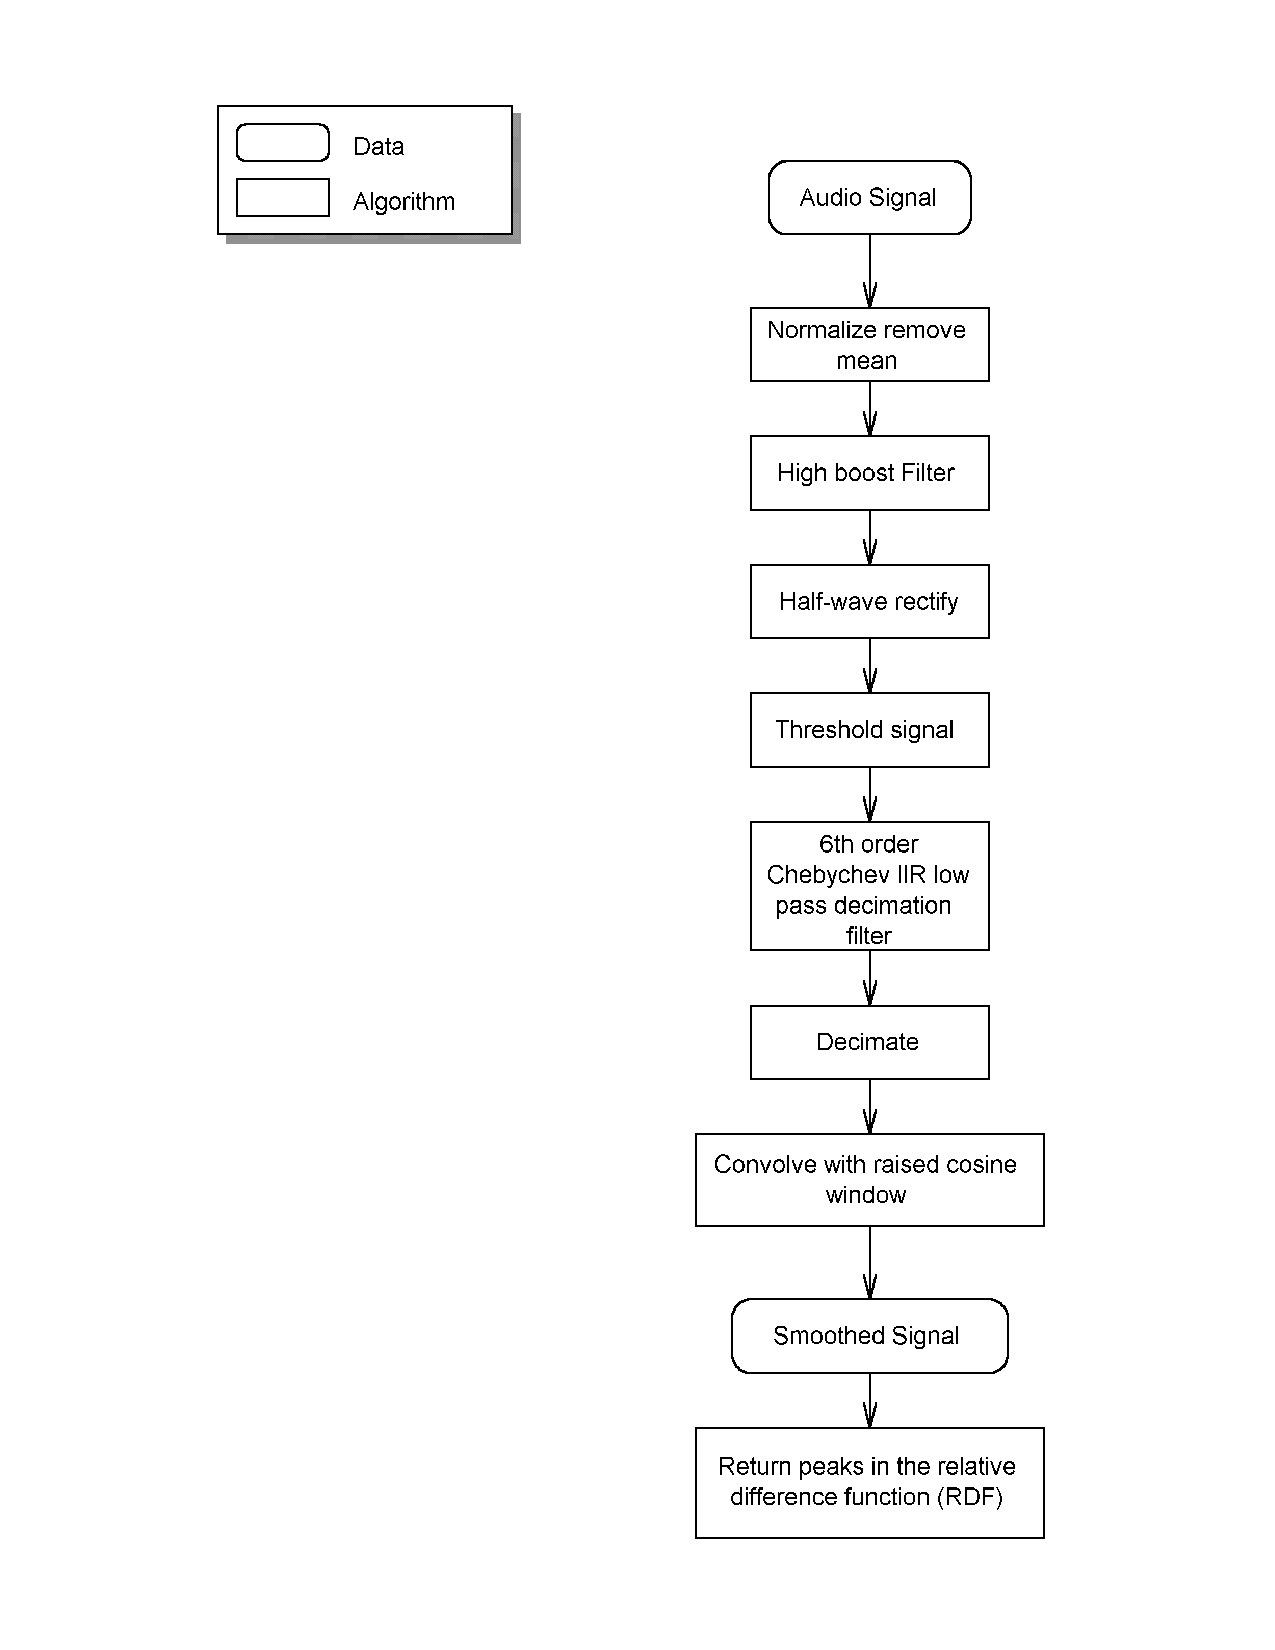
\includegraphics{OnsetDetectionFin.pdf}}
    \caption{Onset Detection Data Path}
    \label{Onset Detection}
  \end{center}
\end{figure}

%
% The first interpretation of the timing information ...
%
\vspace{7mm}
\section{Determination Of A Per-Stream Lowest Level Pulse}
\vspace{3mm}

% Furthermore any kind of musical information is open to multiple interpretation, 
% automated or otherwise.  With this in mind the ``interpretation'' of the timing
% information in terms will have a main candidate for grid size and other
% auxiliary ones.  This aspect in many previous computational models has been
% ignored because ambiguity is ambiguously represented [cite Desain Can Comp Models]

Having successfully separated individual streams from a sound
mixture, each potentially corresponding to a different instrument or 
sound source, timing information is then extracted. So far, this is 
the first of the two high level functions discussed above. 

The next step is to make rhythmic sense of the timing information.  
For example, with the per-stream time vectors we could try to find 
hierarchical time or grouping structures. We can also try to estimate
the overall and per-stream pulse or if applicable 
estimate quantities like meter and strength of beats. Due to time 
constraints and the limited scope of this thesis, I implemented only 
one interpretive module, one that estimates the lowest level pulse per-stream.

This idea of each stream having its own pulse is a deviation from all
previous work in the field which has tried, given a piece of music, to
estimate the {\it overall} lowest level pulse \cite{Scheirer:98tempo}.
If, however, pulse information is clearly determined for {\it each} 
instrument in an ensemble, then it is possible to examine a variety 
of sophisticated rhythmic inter-relationships between instruments.

\vspace{5mm}
\subsection{The Greatest Common Divisor (GCD) of the IOIs}

The algorithm I used to determine the per-stream pulse was
incidentally also from Tampere University of Technology (TUT), 
this time by Jarno Sepp\"anen. It is based on finding the 
``temporally shortest and perceptually lowest-level pulse''
\cite{Seppanen:99}. This idea of a temporal atom is not new 
and has been suggested by others as tatum, quantum or clock \cite{Seppanen:99}\cite{Bilmes:93}. 
Estimating the tatum of a piece of music is equivalent to approximating the 
greatest common divisor (GCD) of the all the inter-onset intervals (IOI) 
present in the music. 

First some definitions, the GCD of a set of natural numbers $a_i, i
\in I$ is defined to be the largest integer which divides all $a_i$ with a
zero remainder: 
\begin{equation}
gcd(a_1,a_2,...a_n) = max \{d: \forall i \in I: a_i \bmod r = 0 \}
\label{gcd}
\end{equation}
There is a problem however. The inter-onset intervals that are
calculated are not always integral. This is because we are
dealing with real performance data, there are never any such
guarantees. Sepp\"anen suggests that we try to find a tatum that
adequately divides all the IOIs and then define an error function
whose local minima represent the best candidates for the GCD. The
error function proposed is defined as such
\begin{equation}
e(q) =  \sum_{i}[(o_i + q/2) \bmod q - q/2]^2
\label{errorfunc}
\end{equation}
It is loosely based on the error function of the form
$\sum_{i}(o_{i}\bmod q)^2$. So if a GCD exists then the remainder
function will be zero at the GCD, otherwise the best approximation of
the GCD will be the the greatest value $q$ where $e(q)$ has a local minimum.
An assumption made by the remainder function is that IOI deviations
are gaussian in nature. Barring expressive timing modulations,
Scheirer has shown experimental evidence that timing deviations tend to be
distributed normally \cite{Scheirer:98}.

\vspace{5mm}
\subsection{Histogram Representation of Intra Frame IOIs}

Sepp\"anen's algorithm is designed to run in real time, processing data in
frames of 500 msec using a leaky integrator that ``remembers'', with
some decay, data from previous frames.  My implementation of this algorithm
is similar despite its non-realtime operation, because the net effect of listening
to music in realtime to determine a pulse is identical to analyzing a
recording causally.

Because 500 msec analysis frames are a bit short to capture rhythmic modulations, 
a histogram data structure is used to store IOI data from frame to frame.
Each time the histogram data structure is updated with IOI information from
the current frame, the newest additions are weighted higher while
histogram data from previous frames are weighted lower with some decay value. 

As IOI data is accumulated, it is first discretised to be a multiple of
the reciprocal of the sample rate $f_{s}$.  If $f_{s} = 44100$ there will
be $44100$ bins in the histogram each $1/44100$ seconds wide. This also means
that the upper bound on the lowest pulse is one second, as an IOI larger than
one second will ``fall off'' the histogram. This is a valid constraint as it
matches psychological experiments where events that are spaced more than 
two seconds apart are not able to be understood in a rhythmic context \cite{Warren:93}.

As we accumulate IOI data in the histogram form, each bin of the histogram
with a value greater than zero can be seen as an element of a set for which
we must find the GCD.  The error function defined above now must be expressed
in terms of the histogram bin values. Sepp\"anen defines such a function
as $$e(q) ={ \sum_{k=0}^{M-1}h[k][(h_{x} + q/2)\bmod q - q/2]^2 \over
  \sum_{k=0}^{M-1}h[k]}$$ where $h[k]$ is a histogram bin value and
$e(q)$ is normalized by the instantaneous histogram mass $\sum_{k=0}^{M-1}h[k]$. Once the error function is calculated,
the largest indice containing a local minimum is the candidate for
GCD.  Picking this candidate involves a traversal of the error
function, calculating first and second order difference functions and 
finding indicies in the histogram that correspond to peaks in the FOD 
that that have positive SOD values (i.e. concave up) 


\begin{figure}[thp]
  \begin{center}
    \resizebox{4in}{!}{\includegraphics{GCDErrorFunc.pdf}}
    \caption{The error function from one 500 msec frame of onset
      times extracted from the soukous kick drum. The largest indice
      with the lowest local minima is 96. Thus the lowest level pulse
      corresponds to the time in seconds represented by histogram bin 96} 
    \label{The GCD Error Function $e(q)$}
 \end{center}
\end{figure}


As the signal's IOI values are successfully accumulated in the
histogram, the arrival of each new frame triggers an update of the error
function and the estimation of the histogram bin containing the GCD. Accordingly,
over the course of a ten second piece of music as many as 20 estimations will
be made for the lowest level pulse, thus capturing rhythmic feature modulations.
This per-instrument low level pulse trajectory is then plotted over
incrementally for the duration of the musical segment in question.


\begin{figure}[thp]
  \begin{center}
    \resizebox{5.2in}{!}{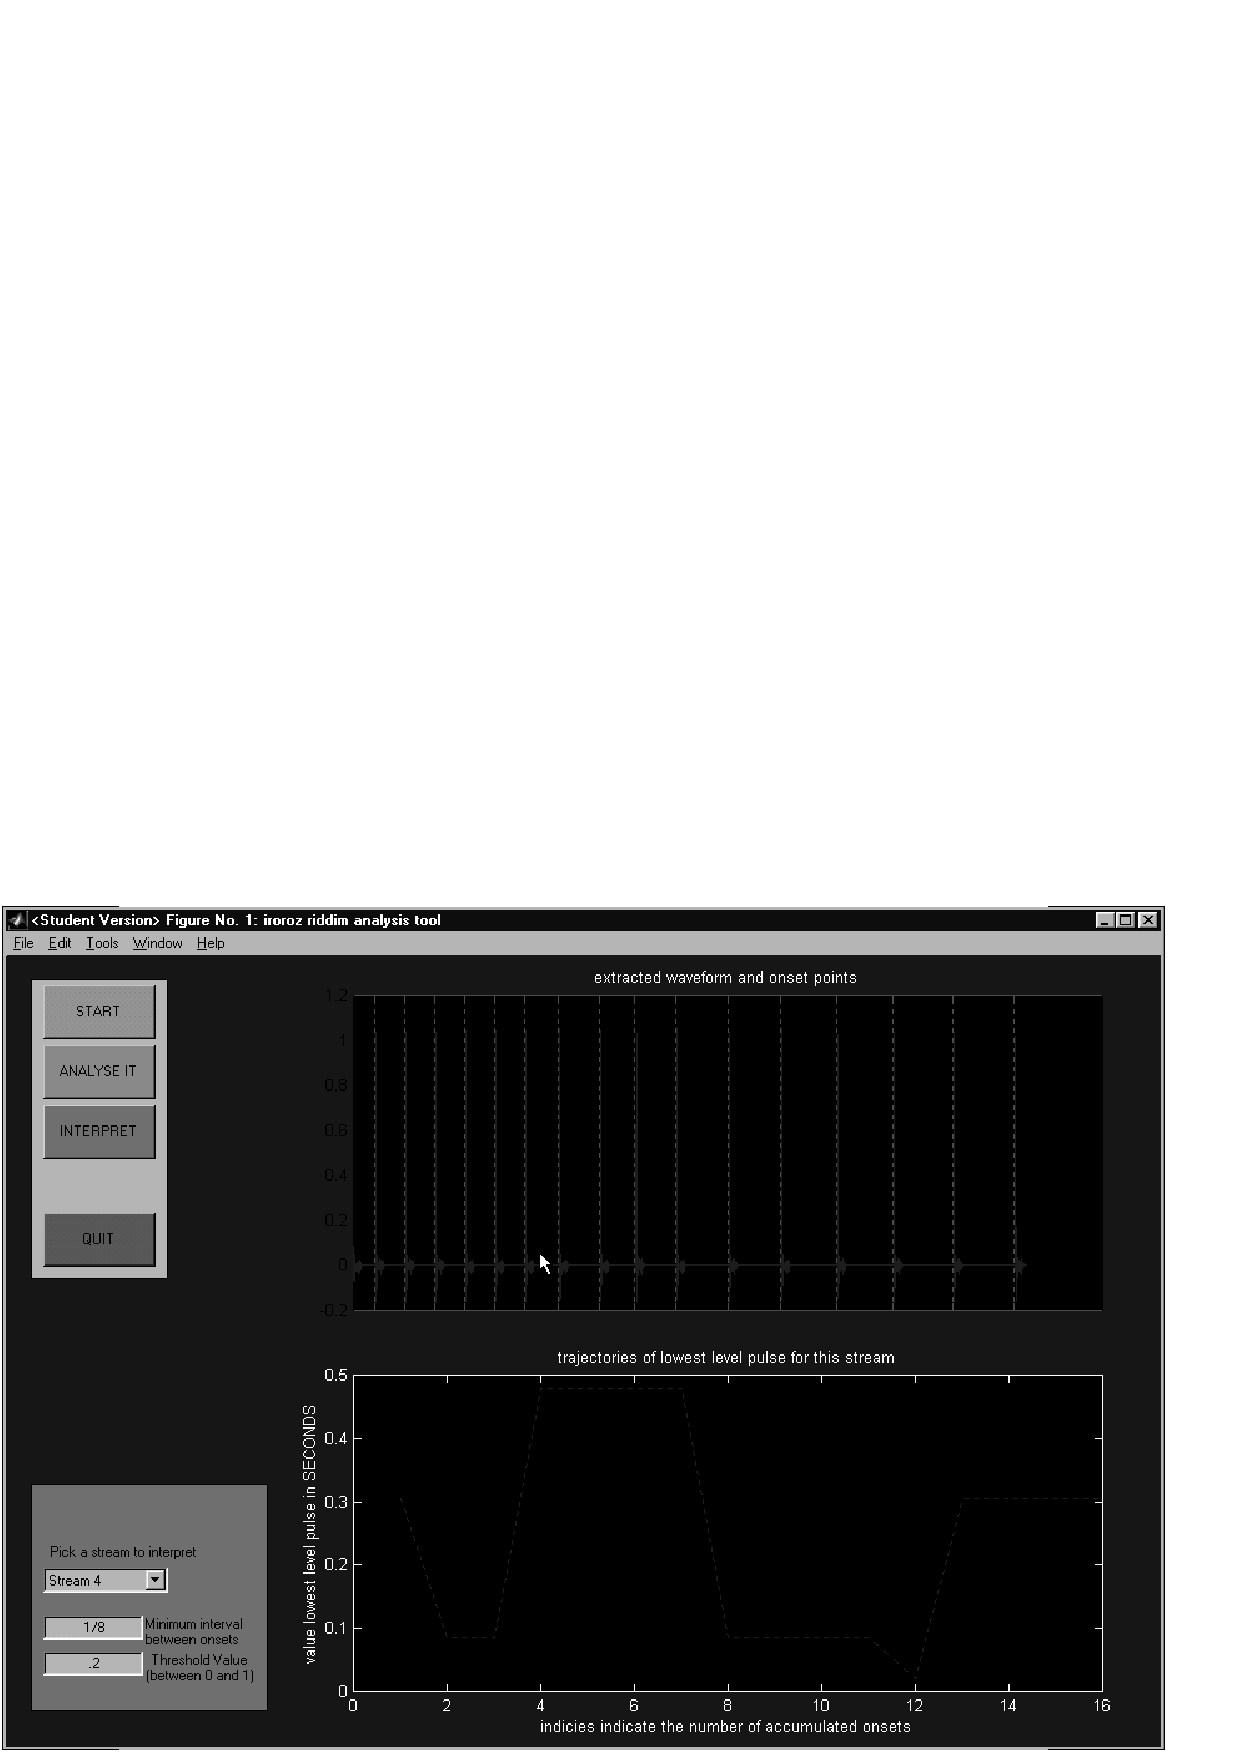
\includegraphics{RiddimScreenInterp.pdf}}
    \caption{A plot of the trajectory of the lowest level pulse}
    \label{lowestlevelpulse}
  \end{center}
\end{figure}